% ============================================================================
% Next-Day Readiness Forecasting in Elite Women's Football
% Generic Overleaf-ready manuscript source
% Compile with pdfLaTeX + Biber (or use latexmk).
% Author details and correspondence e-mail have been populated. See docs/DOI_DEPOSIT_GUIDE.md before submission.
% ============================================================================
\documentclass[11pt]{article}

\usepackage[margin=1in]{geometry}
\usepackage[T1]{fontenc}
\usepackage[utf8]{inputenc}
\usepackage{lmodern}
\usepackage{microtype}
\usepackage{graphicx}
\usepackage{booktabs}
\usepackage{threeparttable}
\usepackage{tabularx}
\usepackage{adjustbox}
\usepackage{float}
\usepackage{placeins}
\usepackage{amsmath}
\usepackage{url}
\usepackage[backend=biber,style=numeric-comp,sorting=none,doi=true,url=true,isbn=false]{biblatex}
\addbibresource{references.bib}
% Compatibility command used throughout the manuscript.
\newcommand{\citep}{\parencite}
\usepackage[hidelinks]{hyperref}

\graphicspath{{figures/}}
\setlength{\parskip}{0.35em}
\setlength{\parindent}{0pt}
\renewcommand{\arraystretch}{1.12}

% Useful project-wide macros
\newcommand{\DeltaMAE}{\ensuremath{\Delta\mathrm{MAE}}}
\newcommand{\Pzero}{\textit{P0}}
\newcommand{\Pone}{\textit{P1}}
\newcommand{\Ptwo}{\textit{P2}}

\begin{document}

\title{Incremental Value of Daily Workload and Wellness Monitoring Beyond a Personalised Readiness-History Baseline for Next-Calendar-Day Readiness in Elite Women's Football}

\author{Haoyang Cheng\\[0.25em]
\small Wuhan Sport University, Wuhan, China\\
\small ORCID: \href{https://orcid.org/0009-0009-4123-2610}{0009-0009-4123-2610}\\
\small Correspondence: Haoyang Cheng, \href{mailto:1303615018@qq.com}{\texttt{1303615018@qq.com}}}
\date{}

\maketitle

\begin{abstract}
\textbf{Purpose:} Daily workload and wellness monitoring are widely used in elite football, but it is uncertain whether a broader daily panel improves short-horizon readiness forecasts beyond current readiness and the player's own prior forecast errors. We evaluated the incremental forecasting value of a daily workload--wellness panel for next-calendar-day self-reported readiness in elite women's football and examined its stability in a two-team transportability assessment under sequential personalisation.

\textbf{Methods:} This secondary longitudinal forecasting analysis used publicly available SoccerMon subjective-monitoring data from 50 players in two elite women's football teams. The paired primary cohort comprised 14,582 player-day pairs with a complete current-day readiness and wellness profile, observed next-day readiness, and the 7-day load history required by the full model. Predictors available by the end of calendar day $t$ were used to forecast readiness at $t+1$. A current-readiness population model (\Pzero) and a full-monitoring population model (\Pone) were separately tuned in three expanding chronological source-team 2020 folds. During 2021 testing, both models received the same reset, past-only, player-specific residual adjustment. Models were evaluated within teams and bidirectionally across teams. The prespecified primary estimand was \DeltaMAE{} = MAE(\Pone) $-$ MAE(\Pzero), with percentile 95\% player-cluster bootstrap confidence intervals.

\textbf{Results:} The full monitoring model did not reduce MAE in any evaluation setting. \DeltaMAE{} was +0.007 (95\% CI $-$0.005 to +0.023) within Team A, +0.018 ($-$0.005 to +0.047) within Team B, +0.022 ($-$0.005 to +0.053) from Team A to Team B, and +0.004 ($-$0.007 to +0.016) from Team B to Team A; positive values indicate higher error for \Pone. Results were directionally consistent across residual-history windows, a reduced-panel comparison, and a wellness-item-missingness sensitivity analysis conditional on observed current- and next-day readiness.

\textbf{Conclusions:} Among report-complete player-days in these two teams, the evaluated daily workload--wellness panel did not demonstrate stable incremental MAE improvement beyond a personalised readiness-history baseline with identical sequential residual updating. This finding concerns a specific calendar-day prediction task and does not imply that workload or wellness measures are causally irrelevant or lack value for communication, clinical reasoning, or other athlete-management decisions.
\end{abstract}

\textbf{Keywords:} athlete monitoring; women's football; readiness to train; training load; wellness; personalised forecasting; transportability

\section{Introduction}
Daily athlete-monitoring systems commonly capture internal training load and self-reported wellness to support training planning and athlete communication \citep{Halson2014,Brink2010,Rago2020,Saw2016,Thorpe2015}. Training duration, rating of perceived exertion (RPE), session-RPE load, sleep, fatigue, soreness, mood, stress, and perceived readiness can be collected repeatedly in field settings. However, repeated self-reporting can impose reporting and data-management demands and frequently produces missing observations, requiring that monitoring studies define the intended decision problem before assuming that a larger panel is necessarily more useful \citep{Saw2016,Midoglu2024}.

A central practical question is therefore not simply whether workload and wellness correlate with readiness. Several studies indicate that wellness responses can vary with training exposure and that dose--response relations may be nonlinear or context-dependent \citep{Campbell2020,Campbell2021}. Rather, the relevant question for day-to-day monitoring is whether a larger panel yields an incrementally better forecast than a strong comparator that already uses the athlete's own recent readiness. If an athlete's preceding readiness reports already capture much of the persistent and short-term information relevant to tomorrow's report, a complex panel may add little forecasting value even when individual panel variables remain meaningful for communication, clinical judgement, or training planning.

This distinction is especially important when monitoring is intended to be individualised. Between-player differences in baseline scores, reporting behaviour, and physical responses can be substantial, and analyses of football performance have shown that monitoring should consider individual variability rather than rely solely on team averages \citep{OlivaLozano2021}. Evidence from women's football should likewise be interpreted in population-specific contexts, because physical match demands and psychological performance factors can vary substantially across female players and competitive environments \citep{Baptista2022,Pettersen2022}. Longitudinal datasets that combine repeated subjective load and wellness reports are valuable for addressing these questions. SoccerMon is notable because it provides openly available repeated subjective and objective monitoring data from two elite women's football teams \citep{Midoglu2024,SoccerMonZenodo}.

Prior work associated with the SoccerMon data stream has shown that readiness trends can be modelled with time-series approaches \citep{Wiik2019,Kulakou2022}. Yet feasibility demonstrations and comparisons of algorithms do not establish whether a full daily monitoring panel improves forecasting beyond a personalised readiness-history baseline, nor whether such value transports from one team to another. The distinction matters because the goal of the present study is prediction rather than causal explanation \citep{Shmueli2010}.

Prediction studies should also be evaluated beyond a single randomly split test set. When the intended use is future forecasting, evaluation should preserve temporal ordering and account for correlated player- and team-level observations \citep{Bergmeir2018,Roberts2017,Debray2023TRIPODCluster}. Calibration is also essential because a model with apparently acceptable error can still produce predictions with inappropriate spread or systematic bias \citep{VanCalster2019,Collins2024}. Cross-team testing further probes whether a model learned from one monitoring environment is transportable to another rather than merely exploiting stable team-specific patterns; performance in a new setting may require updating or recalibration \citep{Janssen2008}.

Accordingly, the primary aim of this study was to assess whether a daily workload--wellness panel adds incremental value beyond a personalised readiness-history baseline for forecasting next-day self-reported readiness in elite women's football. The secondary aim was to evaluate the stability of this incremental-value comparison under within-team temporal validation and bidirectional two-team transportability testing. We hypothesised that any incremental value of the full panel would need to be demonstrated consistently across these settings to be considered practically robust.

\section{Methods}
\subsection{Study design and data source}
This was a secondary longitudinal forecasting analysis of the public SoccerMon dataset \citep{Midoglu2024,SoccerMonZenodo}. SoccerMon contains subjective reports collected from two teams in the Norwegian women's elite football league across the 2020 and 2021 seasons. Training-load reports were completed after training or activity sessions, whereas wellness reports were intended to be completed once per day. The original data collection used the PmSys athlete-monitoring system, was based on written participant consent for open publication, and was approved by the Norwegian Privacy Data Protection Authority (reference 296155) \citep{Midoglu2024}. The present analysis used de-identified public data and did not involve participant contact.

\subsection{Analytic unit, target, and eligibility}
The analytic unit was a player-day pair. For player $i$ on calendar day $t$, all predictors available no later than day $t$ were used to forecast readiness at day $t+1$ (Figure~\ref{fig:design}). The target was the next-calendar-day self-reported readiness-to-train score, recorded on a 1--10 scale. Because the public files provide calendar dates rather than complete within-day timestamps, the design represents a calendar-day forecasting protocol rather than a fully timestamp-verified real-time deployment simulation.

The primary complete-case cohort retained records with complete current-day wellness information, observed next-day readiness, and available 7-day load history, matching the history used by the primary model. It contained 14,582 eligible pairs from 50 pseudonymised players. The player-day eligibility flow and team/year-specific missingness are reported in Figure~\ref{fig:flow} and Supplementary Tables~S4--S5. Because primary eligibility required complete current-day wellness reports, the primary estimand applies to report-complete monitoring days rather than to all calendar days.

\begin{figure}[htbp]
\centering
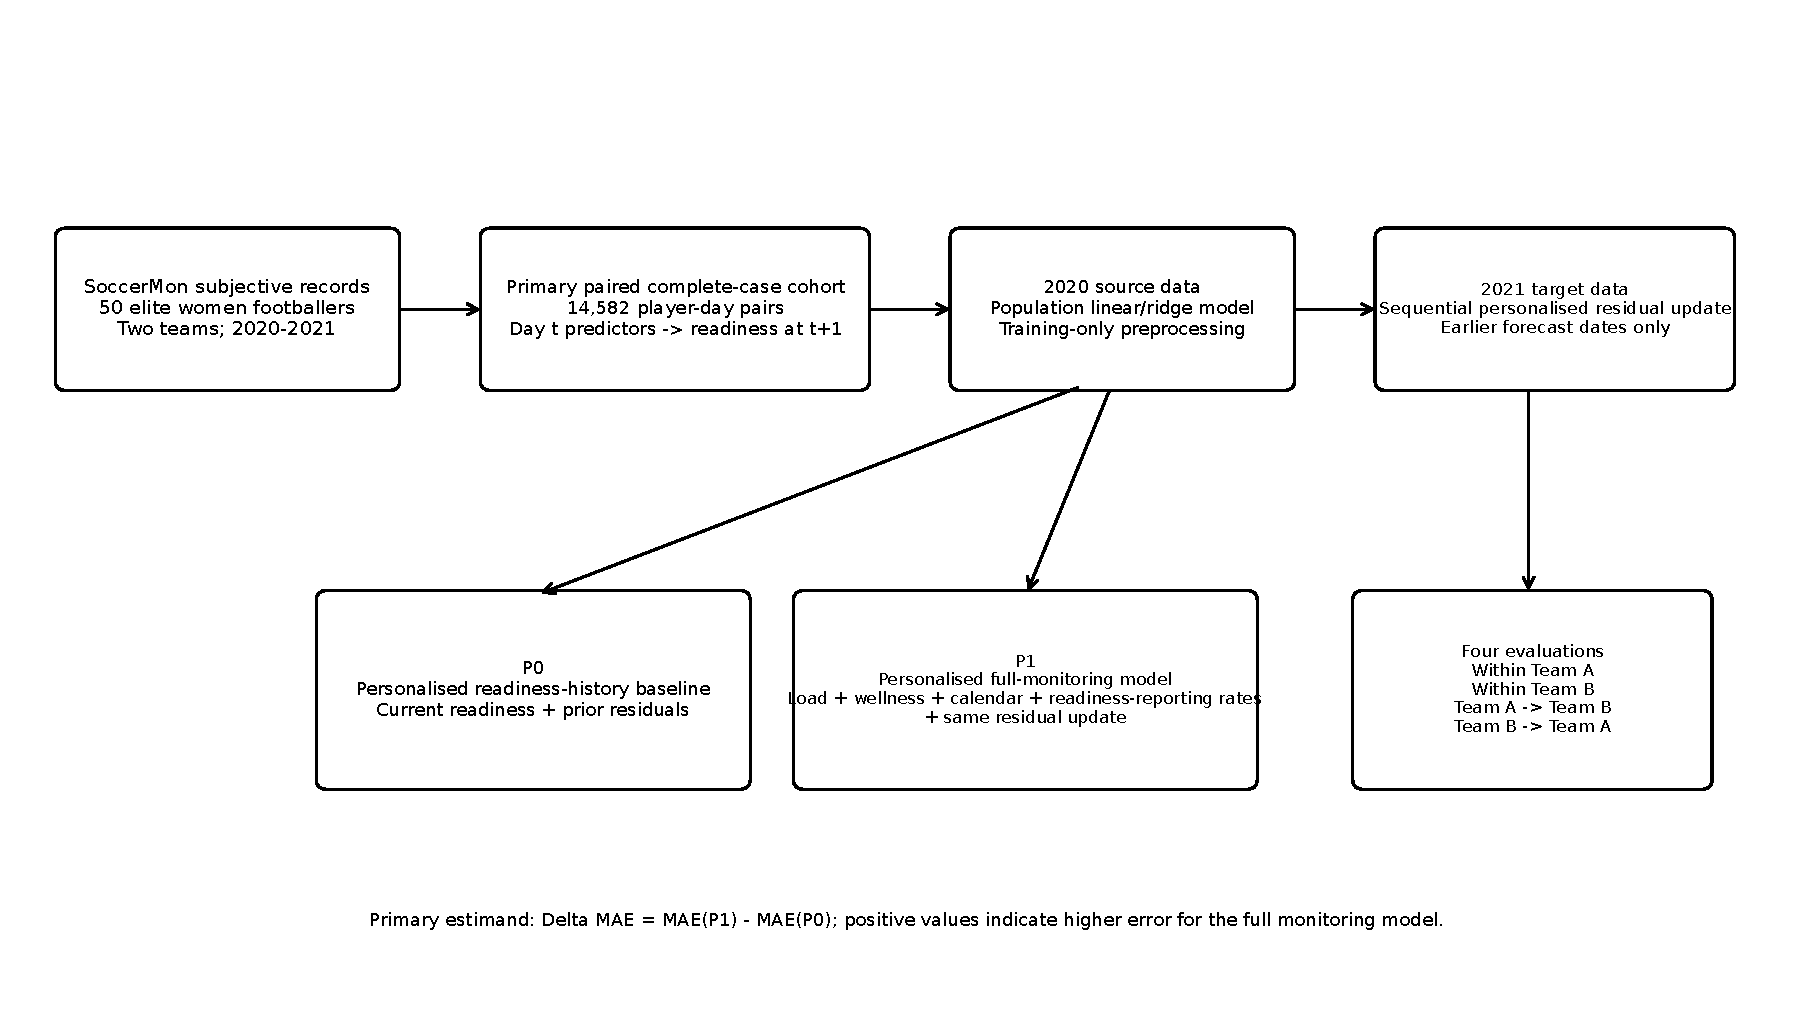
\includegraphics[width=0.95\textwidth]{Figure1_study_design.pdf}
\caption{Study design and leakage-controlled forecasting protocol. Each record was defined at the player-day level. Variables reported no later than calendar day $t$ were used to forecast self-reported readiness at $t+1$. Population models were fitted only to source-team data from 2020. Sequential player-specific residual calibration used only residuals from earlier forecast dates in the target 2021 period.}
\label{fig:design}
\end{figure}

\subsection{Candidate predictors}
The primary comparator, \Pzero, used current-day readiness alone. The full monitoring model, \Pone, used current-day readiness; daily load; 7-day load; the number of training days in the preceding 7 days; current fatigue, mood, sleep duration, sleep quality, soreness, and stress; weekday and month; and recent wellness-reporting density. Daily load was treated as session-RPE aggregated to the player-day level. Load features were log-transformed where appropriate. We deliberately did not simultaneously include a large set of derived workload indicators, such as acute:chronic ratios, monotony, and strain, because these quantities are mathematically related to the same duration and RPE inputs and show substantial collinearity in SoccerMon \citep{Midoglu2024,Rago2020}. A reduced-monitoring model, \Ptwo, was examined in sensitivity analyses and included current readiness, daily load, fatigue, soreness, sleep duration, sleep quality, weekday, and month.

\begin{table}[htbp]
\centering
\caption{Forecasting model specifications.}
\label{tab:models}
\scriptsize
\begin{threeparttable}
\resizebox{\textwidth}{!}{%
\begin{tabular}{p{0.19\textwidth}p{0.47\textwidth}p{0.24\textwidth}p{0.16\textwidth}}
\toprule
Model & Population prediction model & Sequential player adaptation & Role \\
\midrule
\Pzero: adaptive autoregressive baseline & Ridge model using current-day readiness only & Mean residual across the preceding 28 eligible forecast dates for the same player; cold start in the target 2021 period & Primary comparator \\
\Pone: adaptive full-monitoring model & Ridge model using readiness; daily and 7-day load; training-day count; fatigue, mood, sleep duration, sleep quality, soreness, stress; weekday/month; reporting density & Same 28-observation residual adjustment as \Pzero & Primary intervention model \\
\Ptwo: adaptive reduced-monitoring model & Ridge model using readiness; daily load; fatigue, soreness, sleep duration, sleep quality; weekday/month & Same 28-observation residual adjustment as \Pzero & Secondary parsimony sensitivity analysis \\
\bottomrule
\end{tabular}%
}
\end{threeparttable}
\end{table}


\subsection{Population models, chronological tuning, and sequential personalisation}
For each evaluation scenario, linear/ridge population models were fitted only with the designated 2020 source data. Each comparator was tuned separately using three expanding chronological validation folds within the source-team 2020 data. Validation blocks began at approximately 55\%, 70\%, and 85\% of the source team's unique observed 2020 dates. Candidate penalties were $\alpha=0,0.0001,0.001,0.01,0.1,1,10,100,1000,10000,100000$, where $\alpha=0$ denotes the unpenalised linear-model limit.

Tuning evaluated the complete deployment pipeline. For each candidate $\alpha$, a population prediction was generated for a validation block and was then updated using the same past-only sequential residual procedure used in the 2021 evaluations. Residual history was reset at the start of every internal validation block to emulate the target-period cold-start condition. The selected penalty minimised validation-size-weighted MAE of these fully adapted validation predictions; no 2021 target data were used for tuning (Supplementary Table~S1). This design tunes the full deployed comparison rather than only the unadapted population component.

Continuous predictors were median-imputed and standardised using source-data parameters only. Let $\widehat{y}^{(m)}_{i,t+1}$ be the population prediction from model $m$ for player $i$ at time $t+1$. Both \Pzero{} and \Pone{} were then updated by the same online player-specific residual adjustment:
\begin{equation}
\widetilde{y}^{(m)}_{i,t+1} = \widehat{y}^{(m)}_{i,t+1} + \frac{1}{|\mathcal{H}_{i,t}|}\sum_{s \in \mathcal{H}_{i,t}}\left(y_{i,s+1} - \widehat{y}^{(m)}_{i,s+1}\right),
\end{equation}
where $\mathcal{H}_{i,t}$ included up to the 28 earlier eligible forecast dates for the same player in the 2021 target period. At cold start, when no earlier target-period residual was available, the adjustment was zero. This protocol reflects an online monitoring context in which prior observed readiness reports are available, but no future observations are used. It was specified as a light-touch updating strategy for operational monitoring, conceptually related to prediction-model updating in a new setting but not intended as a claim that a universal updating method is optimal \citep{Janssen2008}. The adaptation procedure was deliberately identical for \Pzero{} and \Pone{}, so the primary comparison isolates the incremental contribution of the added monitoring panel beyond the same personal-history information.

\subsection{Evaluation settings}
Four leakage-controlled settings were evaluated: (1) Team A 2020 for training and Team A 2021 for testing; (2) Team B 2020 for training and Team B 2021 for testing; (3) Team A 2020 for training and Team B 2021 for testing; and (4) Team B 2020 for training and Team A 2021 for testing. The cross-team analyses are described as a two-team transportability assessment under sequential player-specific adaptation, not as broad external validation. No random player-day split was used because the intended task was prospective forecasting with clustered repeated observations \citep{Bergmeir2018,Roberts2017,Debray2023TRIPODCluster}.

\subsection{Outcomes and statistical analysis}
The primary performance measure was mean absolute error (MAE). The primary estimand was $\Delta\mathrm{MAE}=\mathrm{MAE}(\Pone)-\mathrm{MAE}(\Pzero)$, so positive values favour the readiness-history baseline. Secondary diagnostics were root mean squared error, mean bias, $R^2$, the percentage of predictions within $\pm1$ readiness point, and the intercept and slope from linear regressions of observed on predicted readiness. We used 2,000 player-cluster bootstrap resamples to obtain 95\% confidence intervals for $\Delta\mathrm{MAE}$. These intervals quantify uncertainty across players within the evaluated target team; they do not represent sampling uncertainty across a population of teams. No smallest practically important MAE difference was prespecified; results therefore compare predictive error and uncertainty rather than formally test equivalence or clinical utility.

Sensitivity analyses varied the residual-history window (14, 28, and 56 prior forecast dates), evaluated \Ptwo, and fitted a missingness-aware full model using source-training median imputation plus wellness-specific missingness indicators in the broader cohort with observed current and next-day readiness and 7-day load history. Analyses were performed in Python using pandas, scikit-learn, NumPy, and Matplotlib. The full workflow, environment specification, and validation checks are archived in the versioned reproducibility package cited in the Code availability statement.

\section{Results}
\subsection{Analytic sample}
The primary file contained 14,569 eligible player-day pairs from 50 players. Team A contributed 3,812 pairs in 2020 and 5,881 in 2021, while Team B contributed 2,393 and 2,483 pairs, respectively (Table~\ref{tab:sample}; Figure~\ref{fig:sample}). Across all pairs, both current-day and next-day readiness had a median of 7.0 (interquartile range 6.0--8.0). The median daily load was 350 session-RPE units (interquartile range 20--600), and 75.0\% of eligible pairs occurred on days with non-zero training load.

\begin{table}[htbp]
\centering
\caption{Analytic sample by team and year. Player counts are reported within team-year strata and are not additive across years.}
\label{tab:sample}
\scriptsize
\resizebox{\textwidth}{!}{%
\begin{tabular}{lccccc}
\toprule
Measure & Team A 2020 & Team A 2021 & Team B 2020 & Team B 2021 & Overall \\
\midrule
Players contributing eligible pairs & 23 & 27 & 14 & 23 & 50 \\
Eligible player-day pairs & 3,812 & 5,881 & 2,406 & 2,483 & 14,582 \\
Current readiness, median [IQR] & 7 [6, 8] & 7 [6, 8] & 7 [6, 8] & 7 [6, 8] & 7 [6, 8] \\
Next-day readiness, median [IQR] & 7 [6, 8] & 7 [6, 8] & 7 [6, 8] & 7 [6, 8] & 7 [6, 8] \\
Daily load (sRPE), median [IQR] & 360 [150, 630] & 320 [20, 560] & 360 [0, 560] & 360 [0, 630] & 350 [12, 600] \\
Pairs with non-zero daily load, n (\%) & 3,100 (81.3) & 4,415 (75.1) & 1,766 (73.4) & 1,657 (66.7) & 10,938 (75.0) \\
7-day readiness-reporting rate, median [IQR] & 1.00 [0.86, 1.00] & 1.00 [0.86, 1.00] & 1.00 [0.86, 1.00] & 0.86 [0.71, 1.00] & 1.00 [0.86, 1.00] \\
\bottomrule
\end{tabular}%
}
\end{table}


\begin{figure}[htbp]
\centering
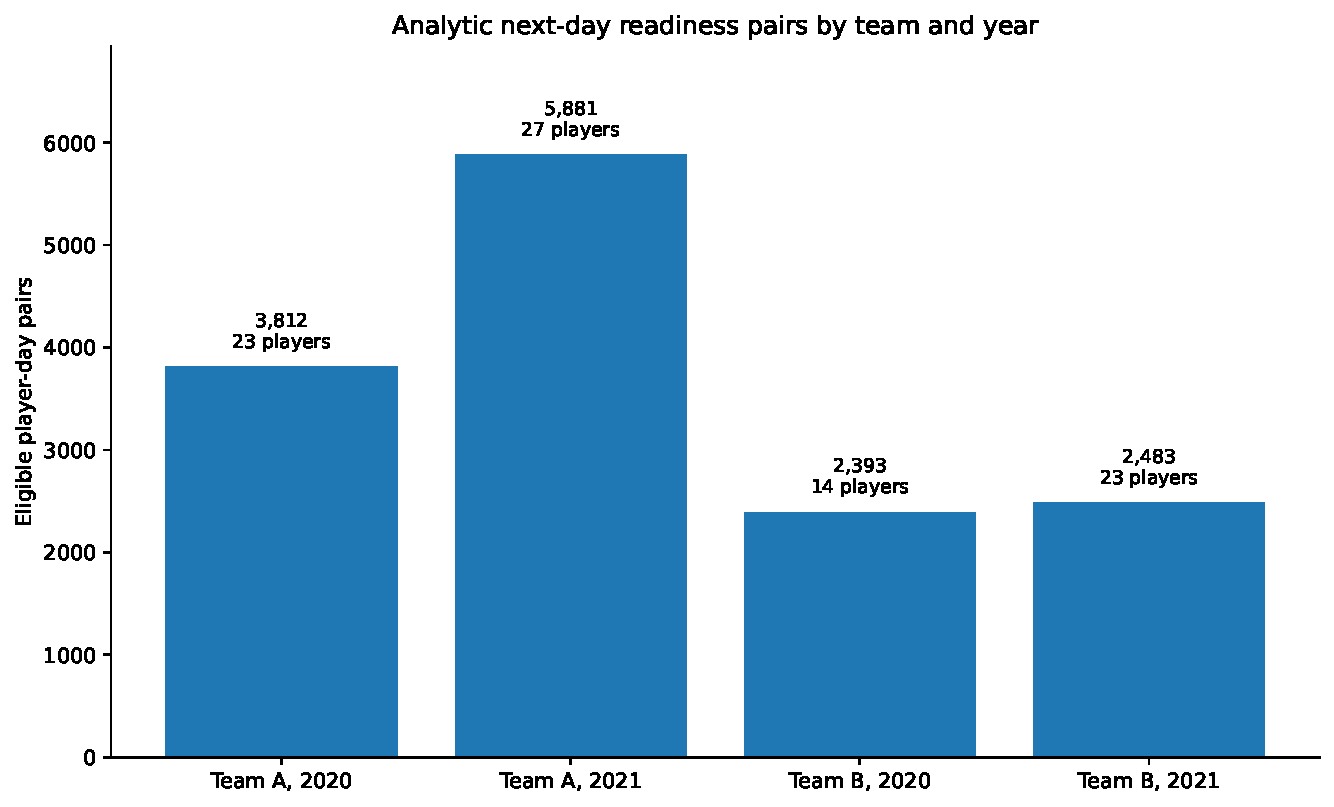
\includegraphics[width=0.75\textwidth]{Figure2_analytic_sample.pdf}
\caption{Analytic sample by team and year. Bars show the number of eligible player-day pairs with complete current-day wellness data and observed next-day readiness. Labels report contributing players in each team-year subset.}
\label{fig:sample}
\end{figure}

\subsection{Primary incremental-value comparison}
Under the primary 28-observation sequential residual window, \Pone{} did not improve MAE over \Pzero{} in any evaluation setting (Table~\ref{tab:primary}; Figure~\ref{fig:incremental}). Within Team A, \Pzero{} and \Pone{} had MAEs of 0.722 and 0.738, respectively (\DeltaMAE{} +0.016, 95\% CI $-$0.001 to +0.036). Within Team B, MAE was 0.632 for \Pzero{} and 0.688 for \Pone{} (\DeltaMAE{} +0.056, +0.009 to +0.102). In cross-team evaluation, \DeltaMAE{} was +0.047 (+0.005 to +0.099) from Team A to Team B and +0.025 (+0.007 to +0.043) from Team B to Team A. Thus, three of four player-cluster bootstrap intervals excluded zero in the direction of higher error for \Pone{}, whereas the remaining within-Team-A comparison was close to null.

\begin{table}[htbp]
\centering
\caption{Primary temporal and two-team transportability results using a 28-observation sequential residual-history window. Positive \DeltaMAE{} values indicate higher mean absolute error for \Pone. Cross-team results use sequential player-specific residual adaptation based only on earlier observed target-team readiness reports.}
\label{tab:primary}
\scriptsize
\resizebox{\textwidth}{!}{%
\begin{tabular}{lrrrrrrr}
\toprule
Evaluation setting & Test pairs & Test players & \Pzero MAE & \Pone MAE & \Pone$-$\Pzero MAE (95\% CI) & \Pzero RMSE & \Pone RMSE \\
\midrule
Within Team A: 2020$\rightarrow$2021 & 5,881 & 27 & 0.722 & 0.738 & +0.016 ($-$0.001 to +0.036) & 1.044 & 1.046 \\
Within Team B: 2020$\rightarrow$2021 & 2,483 & 23 & 0.632 & 0.688 & +0.056 (+0.009 to +0.102) & 1.003 & 0.997 \\
Team A 2020$\rightarrow$Team B 2021 & 2,483 & 23 & 0.623 & 0.670 & +0.047 (+0.005 to +0.099) & 0.975 & 0.983 \\
Team B 2020$\rightarrow$Team A 2021 & 5,881 & 27 & 0.734 & 0.759 & +0.025 (+0.007 to +0.043) & 1.072 & 1.076 \\
\bottomrule
\end{tabular}%
}
\end{table}


\begin{figure}[htbp]
\centering
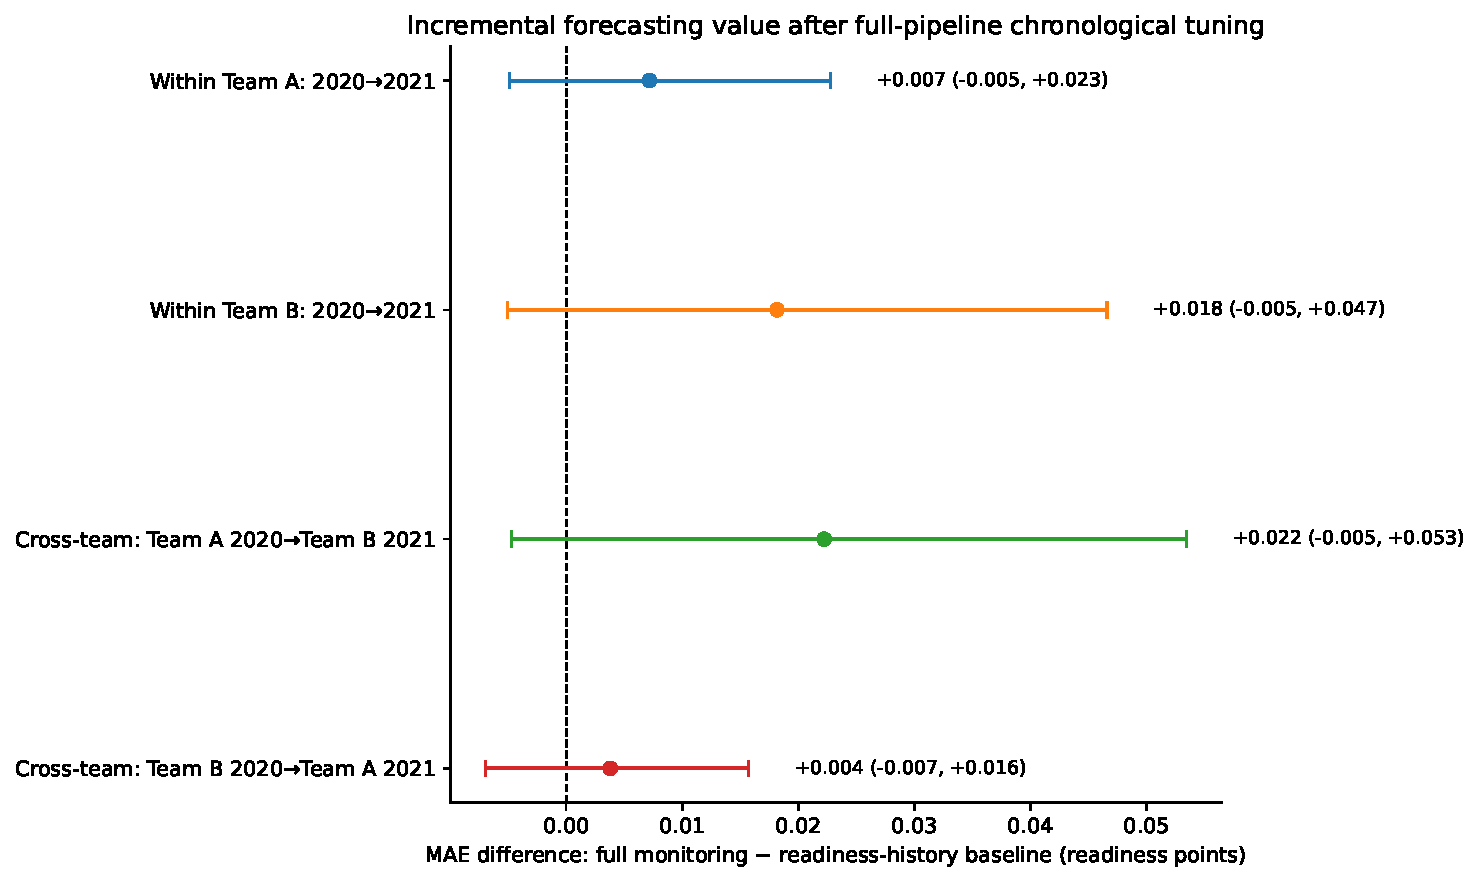
\includegraphics[width=0.90\textwidth]{Figure3_primary_incremental_value.pdf}
\caption{Primary incremental-value comparison. Points and horizontal intervals show player-cluster bootstrap estimates and 95\% confidence intervals for \DeltaMAE{} = MAE(\Pone) $-$ MAE(\Pzero) under the primary 28-observation sequential calibration window. Positive values indicate higher absolute error for \Pone.}
\label{fig:incremental}
\end{figure}

\subsection{Sensitivity analyses and calibration}
Changing the sequential residual window from 14 to 56 earlier eligible forecasts did not reverse the direction of the primary comparison (Figure~\ref{fig:window}; Supplementary Table~S1). Restricting evaluation to observations with 28 available player-specific residuals produced the same directional pattern. The reduced monitoring model \Ptwo{} also did not demonstrate incremental MAE improvement over \Pzero{} (Supplementary Table~S2).

Calibration slopes for both \Pzero{} and \Pone{} were below one in every scenario, indicating that predicted readiness values were somewhat too extreme relative to the observed variation under the stated linear calibration diagnostic (Figure~\ref{fig:calibration}; Supplementary Table~S3). Player-level \Pone{}--\Pzero{} MAE differences varied, but the median difference was positive in every scenario (Figure~\ref{fig:heterogeneity}).

\begin{figure}[htbp]
\centering
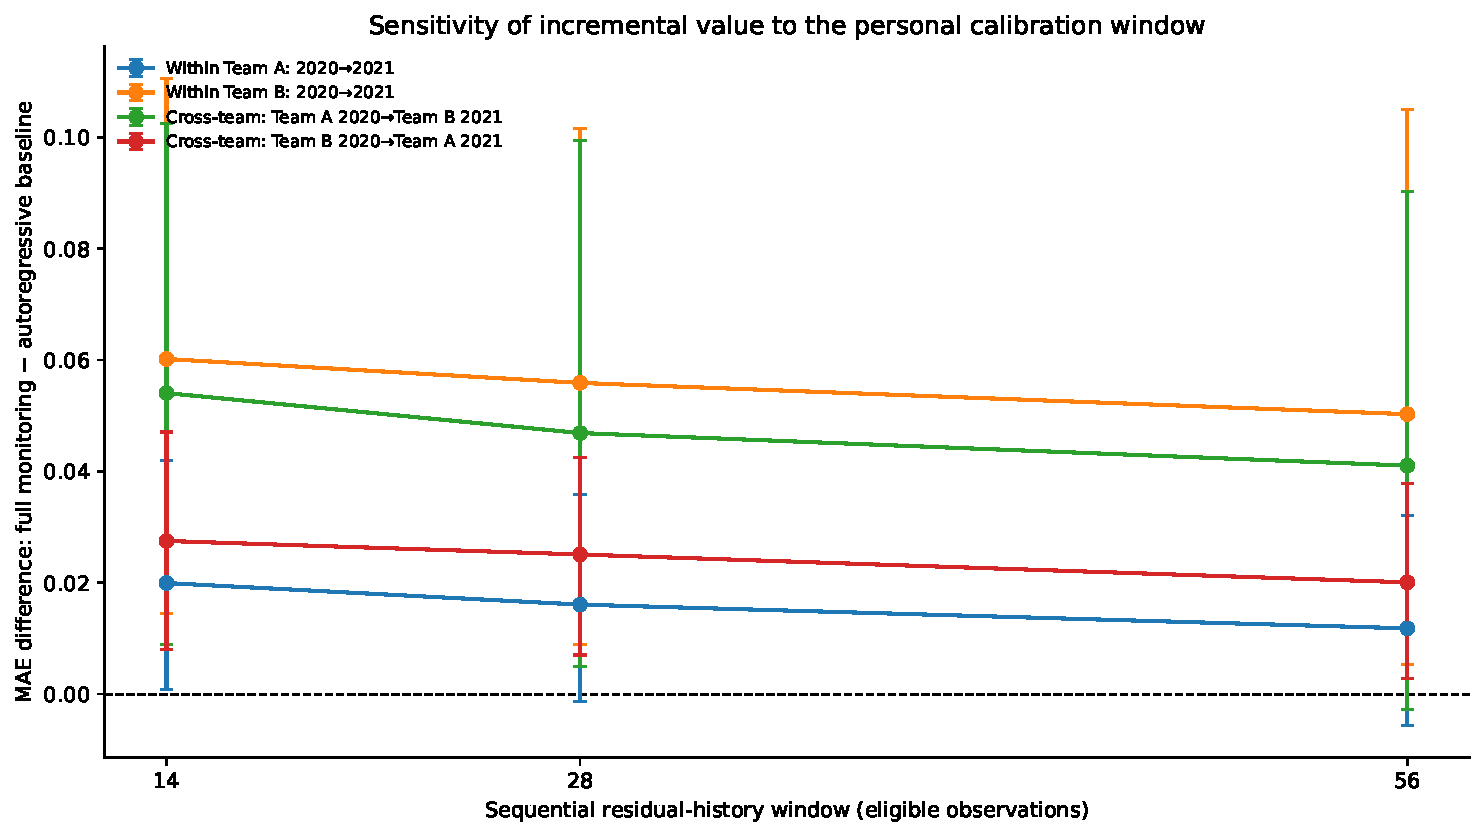
\includegraphics[width=0.90\textwidth]{Figure4_calibration_window_sensitivity.pdf}
\caption{Sensitivity to the residual-history window. Player-cluster bootstrap estimates and 95\% confidence intervals for 14-, 28-, and 56-observation windows. Positive values indicate higher absolute error for \Pone.}
\label{fig:window}
\end{figure}

\begin{figure}[htbp]
\centering
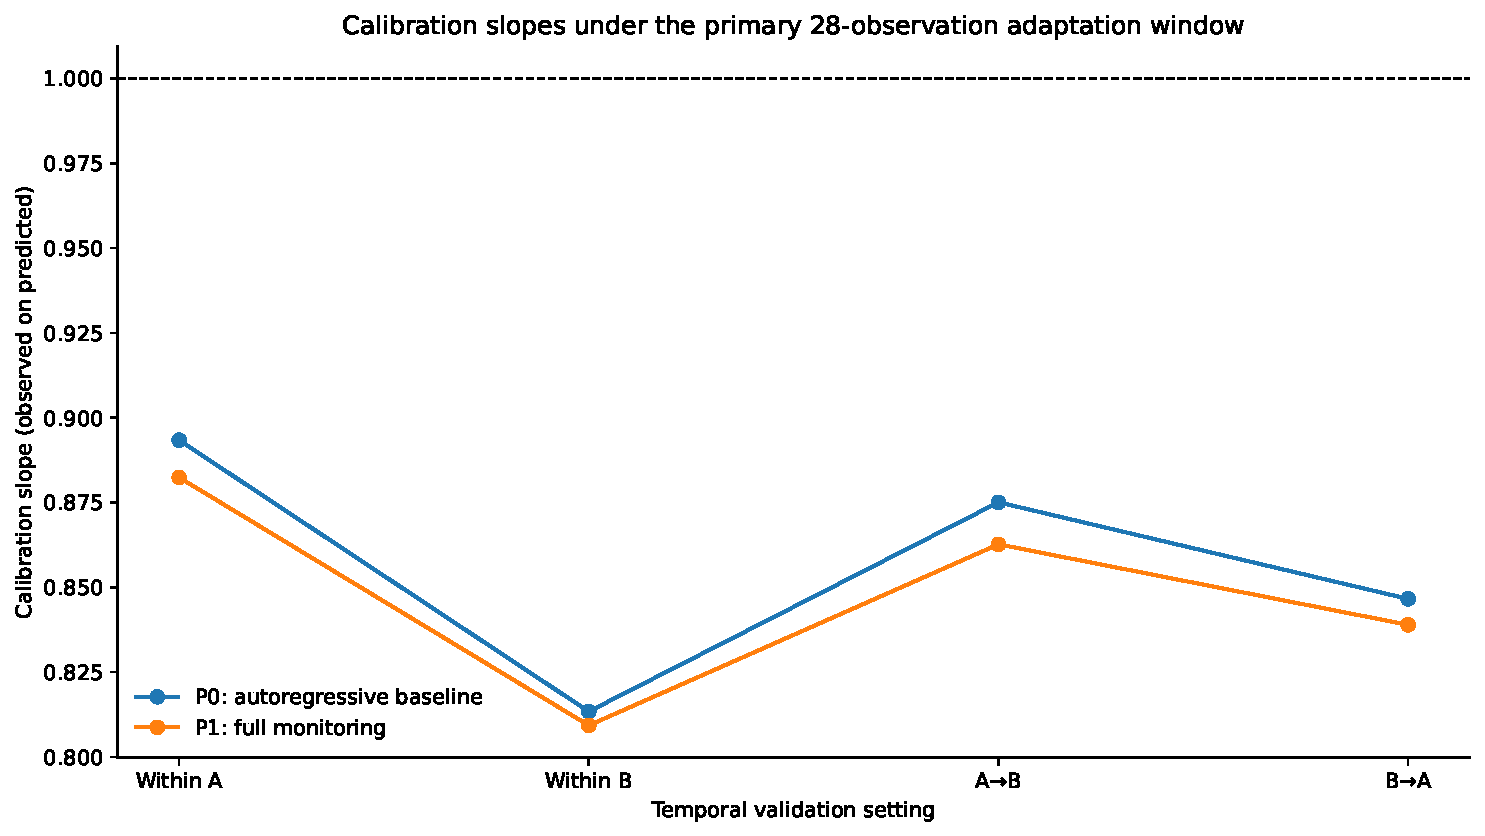
\includegraphics[width=0.90\textwidth]{Figure5_calibration_slope.pdf}
\caption{Calibration slope diagnostic. Calibration slopes were estimated from linear regressions of observed readiness on predicted readiness. The dashed reference is slope = 1.}
\label{fig:calibration}
\end{figure}

\begin{figure}[htbp]
\centering
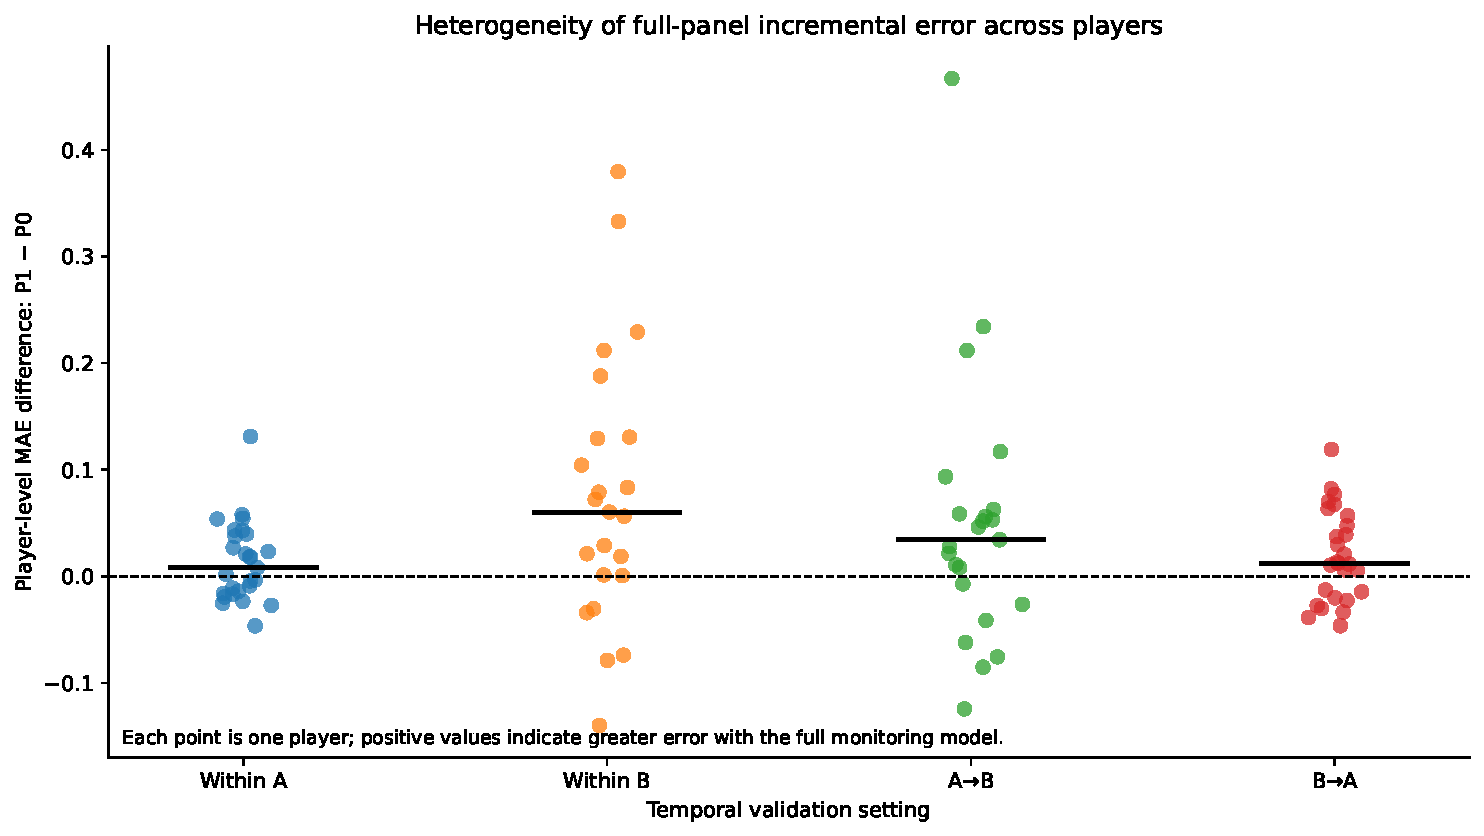
\includegraphics[width=0.90\textwidth]{Figure6_player_level_incremental_error.pdf}
\caption{Player-level heterogeneity. Each point represents one player's \Pone{}--\Pzero{} MAE difference for the primary 28-observation analysis. Positive values indicate higher error for \Pone; black segments denote scenario-specific medians.}
\label{fig:heterogeneity}
\end{figure}
\FloatBarrier

\section{Discussion}
The evaluated daily workload--wellness panel did not demonstrate stable incremental forecasting value beyond a personalised readiness-history baseline. Across two within-team chronological evaluations and two bidirectional cross-team transportability evaluations, the full monitoring model did not lower the prespecified primary metric, MAE, after both comparators had been tuned with the same complete online deployment pipeline. Every player-cluster bootstrap interval for the primary MAE difference crossed zero. The direction of the findings was consistent across alternative residual-history windows, a reduced monitoring panel, and a wellness-item-missingness sensitivity analysis conditional on observed current- and next-day readiness. Because no smallest practically important MAE difference or decision threshold was specified, these findings do not establish formal equivalence, non-inferiority, or absence of all practical value.

The interpretation should remain narrow. The analysis does not show that training load, sleep, soreness, fatigue, stress, or mood are unimportant in athlete management. Such measures may facilitate communication, identify concerns not captured by a single readiness score, support clinical reasoning, or relate to subsequent performance and health outcomes. The present result addresses a specific conditional prediction task: whether the tested daily panel improved next-calendar-day self-reported readiness once the model already had access to current readiness and the same player's earlier prediction errors. In that setting, the added variables did not demonstrate a stable reduction in absolute error.

Several explanations are compatible with this result. First, current readiness may already integrate much of the recent workload and recovery information that players use to report short-term state. Second, the sequential residual adjustment may capture persistent player-specific reporting tendencies and unmeasured contextual influences. Third, individual variables may have useful signal for particular players or situations without providing enough stable, transportable information to improve pooled error across both teams. Finally, self-reported measures collected through the same monitoring system may share response and measurement characteristics, limiting the extent to which a broader questionnaire supplies independent forecast information.

The temporal design is a strength. Random record-level splits can yield optimistic estimates when observations from the same player and team context appear in both development and test samples \citep{Bergmeir2018,Roberts2017}. The present design separated source and target periods and, in two scenarios, source and target teams. The absence of stable incremental gain for \Pone{} under these conditions supports the use of strong personal-history comparators before additional monitoring variables are assumed to add short-horizon predictive value. The cross-team findings nevertheless require careful interpretation. They are a two-team transportability assessment under sequential target-team adaptation, not zero-shot external validation or evidence of universal external validity. In particular, the player-cluster bootstrap intervals quantify uncertainty across athletes within the evaluated target team, not uncertainty across a broad population of teams.

The findings also caution against equating a larger feature set with better short-horizon prediction. Session-RPE and wellness questionnaires can be easy to collect, but routine monitoring has opportunity costs. The appropriate implication is to align measurement burden with a defined decision problem, not to discontinue broader monitoring. When the decision is next-calendar-day readiness forecasting, future work should establish whether each additional measure improves a prespecified error target, calibration, decision utility, or a distinct clinical or performance endpoint.

Several limitations require emphasis. First, readiness was a self-reported 1--10 score rather than an objective performance, clinical, or injury endpoint. Second, the primary paired comparison required complete current-day wellness and observed next-day readiness, so it applies only to report-complete, outcome-observed days. The wellness-item-missingness sensitivity analysis added only 49 player-days and did not address dates on which the daily questionnaire, including current readiness, was not completed. Missingness may be associated with schedule, reporting behaviour, or athlete state; the present design cannot establish how model performance would translate to all calendar days. Third, the sample comprised two teams from one league using one monitoring protocol. Fourth, the analysis used subjective data only; objective external-load variables, match context, menstrual-cycle information, injury status, travel, and other contextual features could alter the incremental-value comparison. Fifth, the models were deliberately parsimonious linear/ridge implementations. Weekday and month were entered as numeric terms rather than as one-hot or cyclic functions, so nonlinear or cyclical calendar effects may not have been fully represented. Sixth, predictions were analysed on a continuous, unbounded scale; an operational system may require a prespecified range-handling rule and evaluation of its consequences. Seventh, the online residual adjustment assumes that earlier target-period readiness outcomes are available. It is appropriate for ongoing monitoring but does not represent a true new-player cold start. Finally, no smallest practically important MAE difference or decision threshold was prespecified. The analyses therefore do not establish formal equivalence, clinical utility, or the causal consequences of changing any monitoring variable \citep{Shmueli2010}.

Future studies should test the same conditional incremental-value question in independent women's football cohorts, include objective external-load and contextual features, explicitly model questionnaire non-completion, assess cold-start performance before residual histories accrue, compare alternative calendar encodings and prediction-boundary rules, prespecify decision-relevant performance thresholds, and evaluate decision-analytic utility. These studies should retain strict temporal alignment, participant-aware validation, calibration assessment, and explicit comparison with strong personal-history baselines \citep{Collins2024,Debray2023TRIPODCluster}.

\section{Conclusions}
For report-complete player-days in two elite women's football teams, the evaluated daily workload--wellness panel did not demonstrate stable incremental MAE improvement beyond a personalised readiness-history baseline with identical sequential residual updating. The result challenges the assumption that routinely adding more daily monitoring variables necessarily improves next-calendar-day self-reported readiness forecasting in this specific calendar-day deployment setting. It does not establish that workload or wellness measures are causally irrelevant, nor does it justify removing them from broader athlete-management practice.

\section*{Practical applications}
\begin{itemize}
\item Evaluate daily monitoring panels against a strong player-specific readiness-history comparator rather than a weak or randomly split benchmark.
\item Report the intended prediction time point, calendar-time validation, calibration, the scope of outcome and questionnaire availability, and the level at which uncertainty is quantified.
\item Treat additional monitoring variables as showing incremental predictive value only when they improve a prespecified decision-relevant outcome; they may still have separate clinical or communication value.
\item Do not infer from this study that teams should stop collecting workload or wellness information. The result is limited to conditional prediction of next-calendar-day self-reported readiness on report-complete days.
\end{itemize}

\section*{Data availability}
The SoccerMon data used in this study are publicly available from Zenodo under a CC BY 4.0 licence: \url{https://doi.org/10.5281/zenodo.10033832}. The original SoccerMon data are not redistributed in this manuscript archive. The analysis code reconstructs the analytic player-day dataset from the official source archive. To avoid duplicate redistribution of player-level data, derived player-day data and individual prediction files are not included in the archive; non-identifying aggregate expected outputs are included for verification.

\section*{Code availability}
The analysis code, manuscript source, figures, tables, and non-identifying reproducibility materials for the v1.1.1 correction release are prepared for archival through Zenodo; the version-specific DOI will be inserted in the post-release submission copy. The public project repository is available at \href{https://github.com/chy010321/next-day-readiness-womens-football}{GitHub}. The release corrects implementation, reporting, and reproducibility documentation; audited primary and wellness-item-missingness estimates were unchanged. The original SoccerMon data must be downloaded separately from Zenodo and are not redistributed in the code archive.

\section*{Ethics statement}
This study was a secondary analysis of publicly available, de-identified data and did not involve direct recruitment, interaction, intervention, or access to identifiable information. No additional ethics approval was obtained for this secondary analysis. The original SoccerMon data collection, including participant consent and applicable ethics and data-protection procedures, is described by Midoglu et al. \citep{Midoglu2024}.

\section*{Use of artificial intelligence}
Generative artificial intelligence tools, including OpenAI ChatGPT (GPT-5.5 Thinking), were used to assist with draft code, language refinement, manuscript organisation, and formatting. All analytical decisions, statistical outputs, reference checks, interpretation, and final manuscript content were reviewed and verified by the author, who takes full responsibility for the accuracy, originality, integrity, and scholarly content of this work.

\section*{Author contributions}
Haoyang Cheng: Conceptualization; Methodology; Software; Data curation; Formal analysis; Validation; Visualization; Writing---original draft; Writing---review \& editing.

\section*{Funding}
This research received no specific grant from any funding agency in the public, commercial, or not-for-profit sectors.

\section*{Competing interests}
The author declares no competing interests.

\section*{Acknowledgements}
The author acknowledges the SoccerMon authors and participating clubs for making the de-identified dataset publicly available.


\printbibliography

\end{document}
